\subsection{Experimental Results}

For the MPC and RAMPC formulated for the same horizon of 10 time steps, \ref{table:} shows the comparison of average tracking cost measured similar to as in equation \ref{}. To get a more accurate picture of how the controllers really performed, we use the following function

\small{
\begin{equation}
J_{true} = \sum_t (x(t)-x_{ref}(t))^{T}Q(x(t)-x_{ref}(t)) + u(t)^{T}Ru(t)
\end{equation}}

Note that since we have access to the true position of the hexrotor with the VICON system, we can obtain the true tracking cost. Table \ref{} also shows the estimated energy consumption based on the time spent in each mode. RAMPC shows better tracking performance than the MPC with either of the 4 fixed modes, showing the improved control performance that can be obtained by dynamically switching between estimation modes in-flight at runtime. Also noticeable in figure \ref{} is how the RAMPC provides better tracking performance, or a lower tracking cost while using lesser energy to do so. This shows that switching between estimation modes improves not only the control performance but also energy efficiency.


\begin{figure}[t]
	\centering
	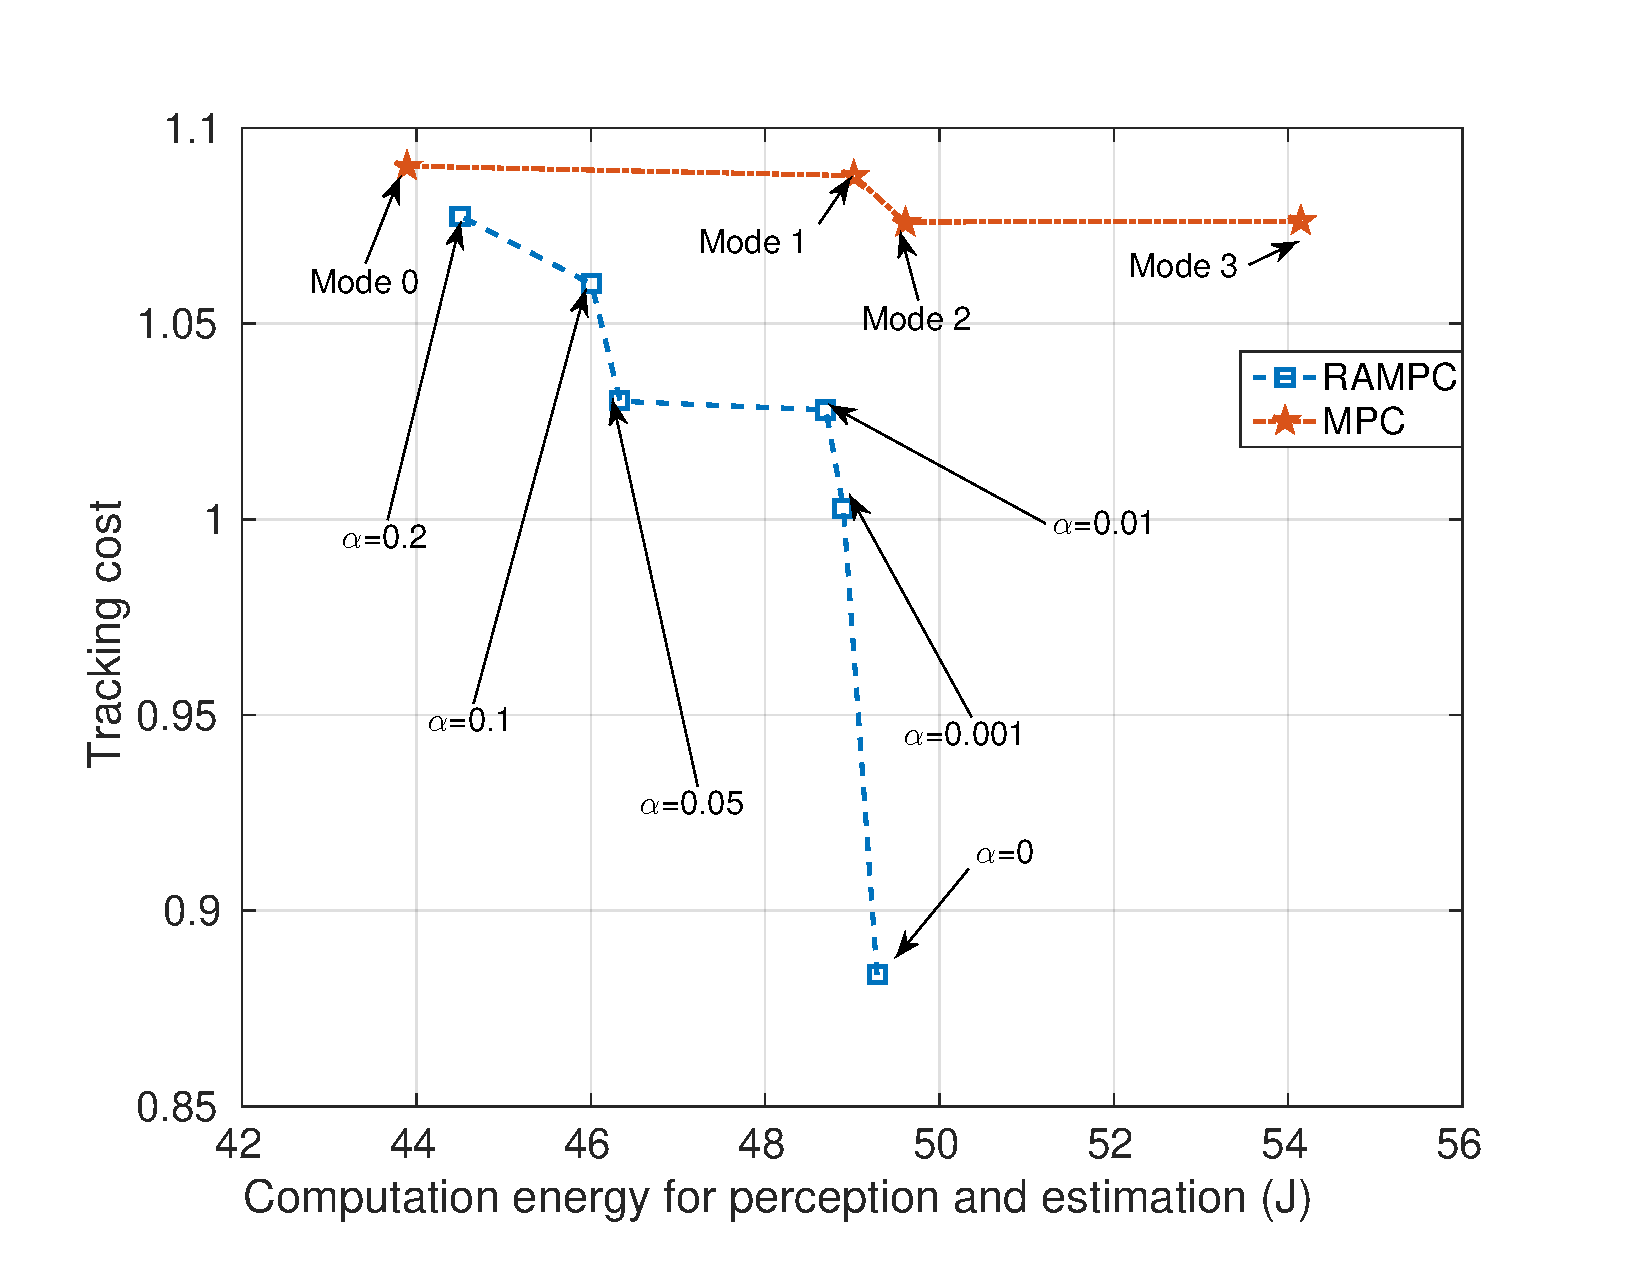
\includegraphics[width=0.9\columnwidth]{figures/TrackingVsEnergy}
	\caption{Tracking cost vs estimated computation energy for executing the perception and estimation algorithm. Note for MPC, different energies are realized only by operating at different fixed modes of the perception and estimation algorithm. Using RAMPC as the controller, the different energies are due to run-time scheduling of different modes based on the optimal value of the cost function \ref{eq: } at each time step based on different values of $\alpha$. It is worth noting that RAMPC with co-design outperforms standard MPC on a tracking performance per unit energy throughout.}
	\label{fig:modeSwitching}
\end{figure}




Figure \ref{} shows the degradation in tracking performance and improvement in energy efficiency as the weight for the energy in the cost function, $\alpha$ is increased (see equation \ref{}). This is expected as with more weight to the energy consumption, the RAMPC switches more often to the low energy (and faster) but less accurate mode 0, as is seen in table \ref{} which shows the fraction of time spent in the 4 modes with RAMPC as $\alpha$ changes.
